%% LaTeX2e class for student theses
%% thesis.tex
%% 
%% Karlsruhe Institute of Technology
%% Institute for Program Structures and Data Organization
%% Chair for Software Design and Quality (SDQ)
%%
%% Dr.-Ing. Erik Burger
%% burger@kit.edu
%%
%% See https://sdq.kastel.kit.edu/wiki/Dokumentvorlagen
%%
%% Version 1.4, 2023-06-19

%% Available page modes: oneside, twoside
%% Available languages: english, ngerman
%% Available modes: draft, final (see README)
\documentclass[twoside, english, final]{sdqthesis}

\usepackage[nocn]{ffcode}
\usepackage{csquotes}
\usepackage{float}
\usepackage{geometry}

\ifdraft{
\usepackage{draftwatermark}
\SetWatermarkAngle{50}
\SetWatermarkLightness{0.9}
\SetWatermarkScale{1}
\usepackage{todonotes}
}{}


%% ---------------------------------
%% | Information about the thesis  |
%% ---------------------------------

%% Name of the author
\author{Lars Weber}

%% Title (and possibly subtitle) of the thesis
\title{Generation of Checkpoints for Hardware Architecture Simulators}

%% Type of the thesis 
\thesistype{Bachelor's Thesis}

%% Change the institute here, ``KASTEL'' is default
% \myinstitute{Institute for \dots}

%% You can put a logo in the ``logos'' directory and include it here
%% instead of the SDQ logo
% \grouplogo{myfile}
%% Alternatively, you can disable the group logo
% \nogrouplogo

%% The reviewers are the professors that grade your thesis
\reviewerone{PD. Dr. Robert Heinrich}
\reviewertwo{Prof. Dr. Ralf H. Reussner}

%% The advisors are PhDs or Postdocs
\advisorone{M. Sc. Sebastian Weber}
%% The second advisor can be omitted
\advisortwo{PD. Dr. Robert Heinrich}

%% Please enter the start end end time of your thesis
\editingtime{13. Mai 2024}{13. September 2024}

\settitle

%% --------------------------------
%% | Bibliography                 |
%% --------------------------------

%% Use biber instead of BibTeX, see README
\usepackage[citestyle=numeric,style=numeric,backend=biber]{biblatex}
\addbibresource{thesis.bib}

%% For example texts -- please remove in the final version
\usepackage{blindtext}

%% ====================================
%% ====================================
%% ||                                ||
%% || Beginning of the main document ||
%% ||                                ||
%% ====================================
%% ====================================
\begin{document}

\newcommand{\todonote}[1]{\ifdraft{
\todo{#1}
}{}}

%% Set PDF metadata
\setpdf

%% Set the title
\maketitle

%% The Preamble begins here
\frontmatter

%% LaTeX2e class for student theses: Declaration of independent work
%% sections/declaration.tex
%% 
%% Karlsruhe Institute of Technology
%% Institute for Program Structures and Data Organization
%% Chair for Software Design and Quality (SDQ)
%%
%% Dr.-Ing. Erik Burger
%% burger@kit.edu
%%
%% Version 1.3.3, 2018-04-17

\thispagestyle{empty}
\null\vfill
\noindent\hbox to \textwidth{\hrulefill} 
\iflanguage{english}{I declare that I have developed and written the enclosed
thesis completely by myself, and have not used sources or means without
declaration in the text.}%
{Ich versichere wahrheitsgemäß, die Arbeit
selbstständig angefertigt, alle benutzten Hilfsmittel vollständig und genau
angegeben und alles kenntlich gemacht zu haben, was aus Arbeiten anderer
unverändert oder mit Änderungen entnommen wurde.}
 
 
%% ---------------------------------------------
%% | Replace PLACE and DATE with actual values |
%% ---------------------------------------------
\textbf{PLACE, DATE}
\vspace{1.5cm}
 
\dotfill\hspace*{8.0cm}\\
\hspace*{2cm}(\theauthor) 
\cleardoublepage

\setcounter{page}{1}
\pagenumbering{roman}

%% ----------------
%% |   Abstract   |
%% ----------------
 
%% For theses written in English, an abstract both in English
%% and German is mandatory.
%%
%% For theses written in German, a German abstract is sufficient.
%%
%% The text is included from the following files:
%% - sections/abstract

\includeabstract

%% ------------------------
%% |   Table of Contents  |
%% ------------------------
\tableofcontents

\listoffigures

%% -----------------
%% |   Main part   |
%% -----------------

\mainmatter

%% LaTeX2e class for student theses
%% sections/content.tex
%% 
%% Karlsruhe Institute of Technology
%% Institute for Program Structures and Data Organization
%% Chair for Software Design and Quality (SDQ)
%%
%% Dr.-Ing. Erik Burger
%% burger@kit.edu
%%
%% Version 1.5, 2024-02-12

\chapter{Introduction}\label{chap:introduction}
The planning and development of large-scale software infrastructures often encompasses software distributed over many different devices,
which may feature vastly different environments for the code running on them.
Especially devices "out in the field" regularly feature architectures very different from the specifications of x86 or ARM,
which makes them very difficult to predict in system simulations or generally in the early planning stages.
Especially when planning real-time systems,
it is very important to plan the communication between IoT devices and the servers running in the backend.
In these scenarios, the backend often runs on x86, or in more recently implemented systems ARM,
while the external devices feature all kinds of different architectures,
that are usually specialized to the task at hand.
Even many IoT devices running ARM cores can often not easily be compared to smartphone- or server-grade ARM.
In addition, when modifying such systems, for example when upgrading hardware,
many of these specialized architectures feature certain behaviors that may be unexpected or not well documented,
which must be addressed when swapping out these physical parts.

In the actual development phase, this issue is already getting solved using emulation.
In the planning phase, especially during design space exploration, where small experiments are already being run,
certain external software is already available, or if the project is a switch of architectures,
like from x86 to ARM in the server world,
emulation could also be used to offer more detailed planning
like for performance criteria.
When a server in a data center is supposed to communicate with an external part that uses pre-developed software,
such an emulation can now be used to produce a good estimate of how performant the server needs to be and how long it should expect to wait for replies.
However, there are issues with emulation, which hinder the use of it in these stages.
The biggest of which is speed, as emulation may result in a slowdown of the factor 1000-10000\cite{slowdown}.
Especially during the exploration of the design space, where only the outline of the project needs to be put down,
such a slowdown is unacceptable, considering the results of the simulation don't need to be exact.

As there are many different emulation environments available,
this thesis chose QEMU, as it is open source and has the most resources available to work with.
The details of the process which led to the selection of QEMU are detailed in \autoref{sec:emulators}.
This thesis tries to generalize findings that may be transferred to other environments,
however as all of these are heavily specialized tools,
the amount of transferrable findings is very limited.

This thesis now introduces the idea of checkpoints to solve this issue of speed and associated resource costs.
The idea is to extract all relevant data from a running emulation
and store it in a generalized way which allows for reusal of the saved state of the system in a different context.
The goal here is to provide a solution with as much flexibility as possible,
meaning a tool which does not require manual tweaking depending on the targeted system.
This especially involves a version-independence in regards to the emulator used.
QEMU has featured the QEMU Human Monitor (QHM) for a long time,
it is however explicitly not meant for processing by other software.
To allow interaction with other software, the QEMU Machine Protocol (QMP) was developed, and the goal is to use this protocol instead,
as the QEMU team tries to keep it somewhat standardized,
while they explicitly write QHM is not stable and there is no guarantee its used formats will be kept consistent,
especially for usages that are not typical for the normal user.
The differences and limitations of both protocols are discussed in detail in \autoref{chap:QEMU_API}.

Initially, this research also aimed to make the development of embedded software easier by using emulation checkpoints to speed up development.
As mentioned before, emulation is very slow.
This of course still applies during development, especially when there is not yet a physical prototype of the developed system available.
To achieve a speedup here, the idea was to make the checkpoints reusable
and create the ability to inject already existing checkpoints back into a running emulation.
This would have even given the option to calculate checkpoints centrally and distribute them,
to save on time and especially resources.
This behavior could not be implemented because of the  limitations of QEMU,
more details on this can be read in \autoref{sec:injection}.
In case someone intends to build up on this and implement the re-injection,
they will find all information regarding such functionality found during this research there.

The theoretical outlines of this thesis including definitions used as well as other works in this field are included in \autoref{chap:Foundations}.
\autoref{chap:QEMU_API} contains both a description of the QEMU APIs according to their official documentation,
however also findings by myself as the official documentation is quite lacking in certain parts, especially the documentation about QHM.
For this reason, it was also decided to make it into its own chapter.
The implementation itself as well as challenges faced during it are mentioned in \autoref{chap:implementation},
and the results of this implementation are discussed and evaluated in \autoref{chap:Evaluation}.
Finally, the works and results of this thesis are concluded in \autoref{chap:Conclusion}.
\chapter{Foundations}
The purpose of this chapter is to lay the groundwork for this thesis
and to establish technical terms used in this writing.
In addition, contradicting definitions get explored
and the process of deciding which ones will be used explained.
The basic technologies involved in this thesis are also adressed in this chapter.

\section{Emulation \& Simulation}
The core of a paper about extracting data from an emulation
to process this data regarding a full system simulation is to fully define these terms,
as they appear very similar.
The importance of a strict definition inside this paper gets even more important
once one starts to actually search for such a definition.
When one starts looking for such a definition,
one will very quickly find one of 2 posts on StackOverflow \cite{SO_link}\cite{SO}.
StackOverflow of course is no reliable source for scientific work,
the reason they are mentioned here is the first one linking to the second one
with the words \enquote{Exactly the opposite answer here:}\cite{SO_link}.
A small discussion, which stays rather civilized for StackOverflow's standards\todonote{Das wieder rausnehmen}, follows,
and people seem to generally agree these terms are heavily subjective and one should clearly define what exactly they're talking about.

This is a small example of showing how there 2 terms are not cleanly defined,
so for this thesis 2 approaches were looked into,
from which a consistent definition inside this thesis is gathered.

\subsection{Emulation \& Simulation according to the Oxford Dictionary}
The Oxford English Dictionary defines the 2 terms as following:
\begin{itemize}
    \item \emph{Emulation:} \enquote{The technique by which a
    computer is enabled, by means of special
    hardware or software, to execute programs
    written for a different type of computer}\cite[p. 196]{emulation_oxford}.
    \item \emph{Simulation}: \enquote{The technique of imitating the behaviour of
    some situation or process (whether economic,
    military, mechanical, etc.) by means of a
    suitably analogous situation or apparatus, esp.
    for the purpose of study or personnel training}\cite[p.503]{simulation_oxford}.
\end{itemize}
From these definititions, one may deduce that emulation is a special case of simulation,
in which an \enquote{apparatus for the purpose of study} is created to \enquote{imitate the behavior of some situation or process},
namely the internal workings of a computer of a different type.\linebreak
The term of \enquote{simulation} instead is easily scaled up or down to suit the current needs.
It may describe a device imitating a large software infrastructure running across many different devices,
perhaps by emulating computers involved in such a system,
however it may also describe the process of imitating the L1-cache of a CPU inside an emulation.\linebreak
This may be concluded by saying that emulation is a special type of simulation,
which itself requires smaller systems of simulation to function,
but can then be used to create bigger systems of simulation.

\subsection{Emulation \& Simulation in scientific literature}
In scientific literature, a search for such a definition does not yield many results.
The closest to a definition in IT comes from \Citeauthor{definition_iot}
while talking about the future chances of the Internet of Things for logistics\cite{definition_iot}.
They explicitly define emulation as a special case of simulation,
and the definitions are generally compatible with the one before.
\begin{itemize}
    \item \emph{Simulation}: A simulator only models and abstracts the system it is simulating.
    This means, in its development decisions must be made as to how precise the simulator works.
    For this, a model must be created and requirements for actual execution developed.
    Later on the results of such a simulation must then be carefully evaluated to make sure
    there are no errors that come from such abstraction
    or are accounted for and get compensated.
    The advantage of such a process is the high speed it carries,
    as simplifications often take away lots of required computation time.
    The disadvantage, as mentioned, however is the potentially high error rate for results,
    and the simulation usually breaking down when trying to analyse small details of a larger system\cite{definition_iot}.
    \item \emph{Emulation}: An emulator is heavily coupled to real components.
    In addition, it's field of work is usually smaller and defined very precisely.
    In return, the results of an emulator are very precise, in most cases exact.
    Error states of the real hardware are also modeled, meaning when feeding it with incorrect data,
    one can observe how the system will behave in abnormal states, which often isn't modeled in a Simulation.
    The big disadvantage of emulation however is its massive cost,
    both in development time and ressources,
    as emulation usually requires a lot more computing power than the device it emulates\cite{definition_iot}.
\end{itemize}

\subsection{Conclusion}\todonote{Think of a better title}
In this thesis therefore Emulation will be viewed as a special kind of simulation,
which perfectly simulates a computing device of a specific architecture
on another computing device, which may or may not be of another architecture.
This especially distinguishes emulation from software like Wine, which is not an emulator\todonote{I really need to stop},
as such software only provides other runtime software a program requires to function, but does not simulate another device in any way\cite{wine}.

In contrast, the abilities of Simulation are much broader,
especially as a simulator may leave out aspects of the real system
its developers don't deem as neccessary for the experiment they want to conduct.
An example of such software in software development is Mockito,
which provides to other parts of a program certain APIs during testing,
which however are not fully implemented yet,
but still return plausible values that allow for testing.

Most people have likely had contact with both these terms in the world of video games,
where they however fulfill completely different jobs.\linebreak
Simulators are usually a type of game,
which allows the player to have an experience he usually does not have in real life.
In a good game, such an experience makes the player feel the imitation is very realistic,
even though it is often simplified heavily.
An example are flight simulators, in which many players feel like they are getting a realistic experience,
even though many features like navigation or communication with Air Traffic Controller are heavily simplified
and can often be turned off.
Which is also an important feature of simulators, the ability to tune the precision
to the current needs to produce a result that is both precise enough for the current problem,
while not wasting resources during uneccessary calculations.\linebreak
Emulators on the other hand get used to allow playing games which were developed for systems which no longer exist.
An example of such an emulator is xemu\cite{xemu},
which we will encounter again later on.
Such emulators perfectly \emph{simulate} the physical hardware of a specific game console,
and allow games compiled for it to run on them.
Xemu for example has to emulate the original Intel Coppermine CPU and Nvidia MCPX X3 GPU
for the games to function, and it must emulate features that may not be needed at all.
For example it always must emulate the SIMD-registers of the CPU, even though a game may not need them.
An additional constraint is performance, the emulator must run at the same speed as the original device,
and any potential performance benefit a modern computer offers is therefore void.
This is because the games are especially developed for such a platofrm,
and the speed of the games is tied to the Frames per Second displayed.
Meaning more frames per second, which usually results in a better experience for the user,
actually cause the game to run faster.

\section{Full System Simulation}
The purpose of this thesis is to produce data which can later on be used inside a \emph{Full System Simulation}.
As however such a simulation is not part of this thesis, this section will only offer a short introduction,
which was mostly lifted from \Citeauthor{kitcheckpoints}\cite{kitcheckpoints}.\todonote{Maybe rephrase this to not make it appear like plagiarism.}

When developing a system, which also requires the development of an operating-system-like
software, the actual hardware may not yet be available for testing
as it often is still in development itself.
Especially when developing embedded devices,
the code develeoped for it often runs on a very low level
and the kernel may take on additional tasks it doesn't on general purpose computers.
To allow for testing of any developed software,
the devices it's supposed to run on must be simulated in its entirety,
with its CPU, RAM, GPU and other external components behaving exactly as they would on the actual device.

Especially such special external components are an issue,
as most emulators provide simplified APIs that are adapted to them being used by a general purpose computer.
For example Hyper-V on Windows does not have the ability to provide a GPU to the guest,
instead Linux has to fallback to \emph{llvmpipe} which provides software rendering.
Other software like VMware and VirtualBox provide heavily simplified GPUs to a guest system,
which are often unable to process 3D rendering by default,
and such a feature must be manually enabled if required.
But even then, there is no option to emulate an actual GPU which may be used on a physical device.
%% LaTeX2e class for student theses
%% sections/content.tex
%% 
%% Karlsruhe Institute of Technology
%% Institute of Information Security and Dependability
%% Software Design and Quality (SDQ)
%%
%% Dr.-Ing. Erik Burger
%% burger@kit.edu
%%
%% Version 1.5, 2024-02-12

\chapter{The QEMU API} \label{chap:QEMU_API}
As the goal of this thesis is to extract data without having to change the code of QEMU,
it is necessary to take a look at the data QEMU offers by itself.
QEMU offers 3 kinds of semi-external APIs: The QEMU Human Monitor (QHM)\cite{qhm-documentation},
the QEMU Machine Protocol (QMP)\cite{qmp-description} and so-called "Internal QEMU APIs"\cite{internal}.

As the name suggests, the internal QEMU APIs are not useful for external use by themselves.
Instead, they can be used when modifying QEMU code and then extracting data by employing GDB or directly by the QEMU process.
As the goal is to use any standard QEMU implementation, these internal APIs will not be regarded further in this thesis.

In the two following sections, both QMP and QHM are further explored. Both the basic functionality,
as well as the commands used for this thesis are explained in detail.
Also, the differences between both protocols, especially regarding their capabilities,
are discussed.

\section{QEMU Machine Protocol (QMP)} \label{sec:QMP}
\enquote{The QEMU Machine Protocol (QMP) is a JSON-based protocol which allows applications to control a QEMU instance}\cite{qmp-description}, as described in the QEMU Wiki.
The protocol was merged into the main branch of QEMU in version 0.13 in 2010, however to this day its status remains as "experimental"\cite{qmp-merge}.
The goal was, and still is, to provide the same data QHM provides, but in a format more accessible for machines.

However, this process is far from complete. To give an example, the patch to add the ability to read register contents was only introduced in 2021,
but to this day it hasn't been merged into the mainline branch.
In addition, this patch doesn't actually provide a valid JSON object, but just passes the return of the QHM-command "info registers" into the "result"-string\cite{qmp-registers-patch},
which is also the reason why it was not merged, as it would have been in conflict with the goal of making QMP both machine-readable and externally consistent.

This effectively means QMP is the preferred protocol for performing any given task,
since its outputs are easily parseable and the QEMU team tries to keep them consistent.
However, there are many tasks QMP cannot (yet) perform,
so certain tasks require the usage of QHM for lack of QMP support.
This directly leads to the most important command\cite{qmp-commands}:

\paragraph{human-monitor-command}
This command is rather special, as it doesn't provide any information by itself,
but instead allows for usage of the legacy QHM inside of QMP,
which gives access to a lot more data not yet accessible directly in QMP.
The QEMU reference explicitly marks this command as a \enquote{stop-gap} until all QHM-commands have their counterpart in QMP,
but, as mentioned before, that is not a priority at the moment.
Still, it's currently the only way to access certain data like register contents, even if the results require extensive and complicated parsing.
Further details on how this command is used and what its capabilities are are described later on in \autoref{sec:QHM}.

\paragraph{qmp\_capabilities}
This command must be sent at the beginning of any QMP session to activate the session.
On an unmodified QEMU instance, it returns an empty JSON object.
The command is intended to show the client additional features of a modified QEMU-instance,
however in this thesis this command serves no purpose except unlocking QMP.

\paragraph{query-cpus-fast}
Gives information about all available CPUs, namely their architecture,
their count, and the ID of the host thread simulating the CPU.
The command is a replacement for \emph{query-cpus}, which was removed and returned slightly different data.
The main purpose this command serves for this thesis is to get the CPU count,
as registers need to be queried individually for each CPU.

\paragraph{query-block}
Queries for all kinds of drives. Gives information about attached storage mediums and where their content is stored.
This gets used to back up the necessary files later on.
Also shows empty devices like optical drives which currently don't contain any media.

\paragraph{dump-guest-memory}\label{dump_memory}
This command dumps the contents of the guest's memory to disk.
The command itself offers many options, however most of these don't work.
In the used implementation, the only output format working is ELF, and paging is only possible on x86 guests.
Still, it's the only option in QMP that offers access to the guest's memory.

\paragraph{stop}
Suspends the emulation of the current system. It is necessary to keep the data extracted consistent.

\paragraph{cont}
Continues the execution of a previously paused system.

\section{QEMU Human Monitor (QHM)} \label{sec:QHM}
The QEMU Human Monitor, sometimes referred to as only the QEMU Monitor,
is an interface to send commands to and query data from a running QEMU instance in a human-readable form.
This however often leads to inconsistent representation, as there is no clear standard on how to represent data.
Even within single commands, the format may vary wildly across different architectures or even within the same architecture.
At the same time, documentation of commands is very lacking, sometimes consisting of only a single sentence.
This makes a detailed exploration into their workings necessary, and the results of this research are presented in the following\cite{qhm-documentation}:

\subsection{info tlb}
"info tlb" is described as "Show virtual to physical memory mappings"\cite{qhm-documentation}.
There seems to be no further documentation as to what this command does or the format of the output.
Finding more information about the supposed TLB is also rather difficult.
Most information is therefore derived from the \citetitle{intel-manual},
which therefore only applies to x86 and makes the portability of any information rather questionable.

An example of the output is provided in \autoref{fig:tlb_x86}:

\begin{figure}[H]
\begin{ffcode}
    0000000000010000: 00000000001a0000 ---DA---W
    0000000000011000: 0000000000181000 ---DA---W
    0000000000012000: 0000000000182000 ---DA---W
    0000000000013000: 0000000000183000 ---DA---W
    0000000000014000: 0000000000184000 ---DA---W
    0000000000015000: 0000000000185000 ----A---W
    0000000000016000: 0000000000186000 ---DA----
    0000000000017000: 0000000000187000 ----A---W
    0000000000018000: 0000000000188000 ----A----
    0000000000019000: 0000000000189000 ----A----
    000000000001a000: 000000000016a000 ----A----
\end{ffcode}
\caption{Output of \emph{info tlb}.}
\label{fig:tlb_x86}
\end{figure}

These are the first eleven lines this command outputs when queried against the XBox emulator "xemu"\cite{xemu}.
The output consists of the linear address shown to the guest OS, the "physical" address, which represents the offset in QEMU's emulated memory region,
and the flags associated with each segment.
As the flags are x86-specific, they are currently not of further interest and just get stored without further processing.

It is important to note the physical address is not the actual address in the QEMU process, but the offset from the base address of said memory region.
To correctly extract the guest RAM, one would now need to find the base address of the memory region the QEMU-process uses to emulate RAM,
and then combine it with the virtual address translation to store memory in the format the guest OS sees it.
This throws up the question of which format the RAM should be stored. In the order it is actually on the hardware, meaning the physical addresses,
or in the order the guest OS sees it, meaning the virtual addresses.

\subsection{info mtree}\label{sec:API_mtree}
This command shows all memory regions which are currently allocated for the guest.
This includes main memory, as well as memory for emulated devices like graphic cards.
These regions are given individual names and are separated by blank lines.
\autoref{fig:mem_ARM} gives an excerpt of an ARM64 guest running on x86,
the full output is shown in \autoref{fig:mem_ARM_full}.

\begin{figure}[H]
\begin{ffcode}
    address-space: I/O
    0000000000000000-000000000000ffff (prio 0, i/o): io

  address-space: gpex-root
    0000000000000000-ffffffffffffffff (prio 0, i/o): bus master container

  address-space: virtio-gpu-pci
    0000000000000000-ffffffffffffffff (prio 0, i/o): bus master container

  address-space: cpu-memory-0
  address-space: memory
    0000000000000000-ffffffffffffffff (prio 0, i/o): system
      0000000000000000-0000000003ffffff (prio 0, romd): virt.flash0
      0000000004000000-0000000007ffffff (prio 0, romd): virt.flash1
      0000000008000000-0000000008000fff (prio 0, i/o): gic_dist
      0000000008010000-0000000008011fff (prio 0, i/o): gic_cpu
      0000000008020000-0000000008020fff (prio 0, i/o): gicv2m
      0000000009000000-0000000009000fff (prio 0, i/o): pl011
      0000000009010000-0000000009010fff (prio 0, i/o): pl031
      0000000009020000-0000000009020007 (prio 0, i/o): fwcfg.data
      0000000009020008-0000000009020009 (prio 0, i/o): fwcfg.ctl
      0000000009020010-0000000009020017 (prio 0, i/o): fwcfg.dma
      0000000009070000-0000000009070017 (prio 0, i/o): memhp container
      0000000009080000-0000000009080003 (prio 0, i/o): acpi-ged
      000000000a000000-000000000a0001ff (prio 0, i/o): virtio-mmio
      000000000a000200-000000000a0003ff (prio 0, i/o): virtio-mmio
      000000000a000400-000000000a0005ff (prio 0, i/o): virtio-mmio
      ...
\end{ffcode}
\caption{Output of \emph{info mtree} for an ARM guest.}
\label{fig:mem_ARM}
\end{figure}

In this example, we see memory for basic I/O functionality, the GPEX-host bridge, the emulated GPU, and "cpu-memory-0".
cpu-memory-0 is special, as the name suggests this may be memory used to emulate the CPU. That however is not the case.
Not only is it much larger than the registers of a single-core CPU could be, but also it's a duplicate.
Further down the output is the following data:

\begin{figure}[H]
\begin{ffcode}
    memory-region: system
    0000000000000000-ffffffffffffffff (prio 0, i/o): system
      0000000000000000-0000000003ffffff (prio 0, romd): virt.flash0
      0000000004000000-0000000007ffffff (prio 0, romd): virt.flash1
      0000000008000000-0000000008000fff (prio 0, i/o): gic_dist
      0000000008010000-0000000008011fff (prio 0, i/o): gic_cpu
      0000000008020000-0000000008020fff (prio 0, i/o): gicv2m
      0000000009000000-0000000009000fff (prio 0, i/o): pl011
      0000000009010000-0000000009010fff (prio 0, i/o): pl031
      0000000009020000-0000000009020007 (prio 0, i/o): fwcfg.data
      0000000009020008-0000000009020009 (prio 0, i/o): fwcfg.ctl
      0000000009020010-0000000009020017 (prio 0, i/o): fwcfg.dma
      0000000009070000-0000000009070017 (prio 0, i/o): memhp container
      0000000009080000-0000000009080003 (prio 0, i/o): acpi-ged
      000000000a000000-000000000a0001ff (prio 0, i/o): virtio-mmio
      000000000a000200-000000000a0003ff (prio 0, i/o): virtio-mmio
      000000000a000400-000000000a0005ff (prio 0, i/o): virtio-mmio
      ...
\end{ffcode}
\caption{Duplicate data for \emph{info mtree} on an ARM guest.}
\label{fig:mem-duplicate}
\end{figure}

This shows that the output above is actually normal system memory accessible to the emulated CPU.
Hence the name "cpu-memory-0", as on multi-socket-systems sometimes not all memory is available to all CPUs.

The size of each memory region is shown by the minimum and maximum address of each region.
As this is a 64bit guest, ffffffffffffffff represents 64bits, which results in a memory size of $2^{64}$Bytes.

Most regions are specialized and the name of the region gives an indication of where to look,
but it isn't actually relevant in most cases.
Because of this, only one special region will be explained:

\paragraph{virt.flash}
There are 2 regions with this name. \emph{virt.flash0} is the basic EFI, which under aarch64 is not included by default.
\emph{virt.flash1} stores EFI variables like the boot order.
The reason these regions are split is \emph{virt.flash1} is writeable, while \emph{virt.flash0} isn't.
The main reason these are interesting is them being backed by files on disk.
This means any changes made to these regions by the guest can be easily read externally by opening those files.
Of course that comes with a massive performance penalty if many accesses to such regions are made.

Additionally, since x86 is often more detailed than other architectures,
the full output of \emph{info mtree} is also shown in \autoref{fig:xemu_full}.

\subsection{info registers}\label{sec:info_registers}
This command returns the contents of all the registers for a given CPU.
It gives a detailed overview of the data, however the level of detail on x86 is much higher than it is for other architectures.
To further illustrate this, in \autoref{fig:registers_x86} and \autoref{fig:registers_ARM} example outputs for this command are provided.

\begin{figure}[H]
  \begin{ffcode}
    CPU#0
    EAX=fd000140 EBX=80035bdc ECX=fd601300 EDX=00000000
    ESI=80035a90 EDI=d0008bf8 EBP=80035c2c ESP=800395f0
    EIP=8001b030 EFL=00000246 [---Z-P-] CPL=0 II=0 A20=1 SMM=0 HLT=0
    ES =0010 00000000 ffffffff 00cf9300 DPL=0 DS   [-WA]
    CS =0008 00000000 bfffffff 00cb9b00 DPL=0 CS32 [-RA]
    SS =0010 00000000 ffffffff 00cf9300 DPL=0 DS   [-WA]
    DS =0010 00000000 ffffffff 00cf9300 DPL=0 DS   [-WA]
    FS =0020 80035bdc 0027cfff 00c09300 DPL=0 DS   [-WA]
    GS =0000 00000000 00000000 00000000
    LDT=0000 00000000 0000ffff 00008200 DPL=0 LDT
    TR =0018 8003b160 00000068 00008900 DPL=0 TSS32-avl
    GDT=     8003b298 00000038
    IDT=     80035e60 00000200
    CR0=8001003b CR2=00000000 CR3=0000f000 CR4=00000610
    DR0=00000000 DR1=00000000 DR2=00000000 DR3=00000000
    DR6=ffff0ff0 DR7=00000400
    EFER=0000000000000000
    FCW=027f FSW=0000 [ST=0] FTW=00 MXCSR=00001fa0
    FPR0=0000000000000000 0000 FPR1=0000000000000000 0000
    FPR2=0000000000000000 0000 FPR3=0000000000000000 0000
    FPR4=0000000000000000 0000 FPR5=0000000000000000 0000
    FPR6=0000000000000000 0000 FPR7=0000000000000000 0000
    XMM00=0000000000000000 0000000041080000 XMM01=0000000000000000 000000004f000000
    XMM02=0000000000000000 00000000cf000000 XMM03=0000000000000000 0000000043a00000
    XMM04=0000000000000000 0000000000000000 XMM05=0000000000000000 0000000000000000
    XMM06=0000000000000000 0000000000000000 XMM07=0000000000000000 0000000000000000
  \end{ffcode}
  \caption{Example Output of \emph{info registers} on an x86 guest.}
  \label{fig:registers_x86}
\end{figure}

\begin{figure}[H]
  \begin{ffcode}
    CPU#0
    PC=0000000000000200 X00=0000000000000000 X01=0000000000000000
    X02=0000000000000000 X03=0000000000000000 X04=0000000000000000
    X05=0000000000000000 X06=0000000000000000 X07=0000000000000000
    X08=0000000000000000 X09=0000000000000000 X10=0000000000000000
    X11=0000000000000000 X12=0000000000000000 X13=0000000000000000
    X14=0000000000000000 X15=0000000000000000 X16=0000000000000000
    X17=0000000000000000 X18=0000000000000000 X19=0000000000000000
    X20=0000000000000000 X21=0000000000000000 X22=0000000000000000
    X23=0000000000000000 X24=0000000000000000 X25=0000000000000000
    X26=0000000000000000 X27=0000000000000000 X28=0000000000000000
    X29=0000000000000000 X30=0000000000000000  SP=0000000000000000
    PSTATE=000003c5 ---- EL1h  SVCR=00000000 --  BTYPE=0    FPU disabled
  \end{ffcode}
  \caption{Example output of \emph{info registers} on an ARM guest.}
  \label{fig:registers_ARM}
\end{figure}

It is immediately apparent this output is not intended for further usage by computers,
but instead used by humans debugging QEMU and does not follow any specified format.
This of course is also stated by the QEMU team\cite{qhm-documentation}.
However, because this is the only way to access registers through an external interface,
this output needs to be made parseable by a computer, and for this,
the following rules are presumed from ARM and x86 in the hope they are valid for the majority of architectures:

\begin{itemize}
  \item The CPU number is specified in the first line, even though the command only returns a single CPU which must be specified beforehand.
  \item Registers are formatted in the scheme \$name=\$content.
  \begin{itemize}
    \item On x86, if the name of the register is shorter than 3 letters, the name gets padded with spaces between it and the equals sign.
    \item Longer names are allowed, however as the names of most standard registers are only 3 letters long, this only applies to more specialized registers.
    \item The content is specified in hexadecimal.
  \end{itemize}
  \item The length of the content gets padded with zeroes at the beginning to indicate the length of the register.
  Since this is in hex, each digit represents 4 bits of register length.
  \begin{itemize}
    \item This assumes all registers are of a length divisible by four.
    However, there are registers where this is not the case, for example $HLT$ or $A20$.
  \end{itemize}
  \item QEMU formats the contents into groups of \emph{some} multiple of 32 bits.
  \begin{itemize}
    \item When the amount of bits in a register is not a multiple of \emph{some} multiple of 32,
    there is no standard whether the remaining bits get put at the back or the front.
    See the floating-point and stack-pointer registers.
  \end{itemize}
  \item 3 different ways to represent flags were encountered:
  \begin{enumerate}
    \item Some flags get put in []-brackets, wherein their letter is written if they're set, otherwise a hyphen is shown.
    \item Other flags, especially multibit flags, get represented like their own register.
    \begin{itemize}
      \item In this case, the amount of digits does not indicate the length of the register and therefore its possible values.
      For example, the $A20$-register is only a single bit, while $CPL$ is 2 bits.
    \end{itemize}
    \item If there is not a dedicated register in the specification,
    but it's up to the implementation to decide,
    for example the FPU on ARM,
    there is no standard in how this is treated.
    \begin{itemize}
      \item For the ARM-FPU, \enquote{FPU disabled} gets explicitly written out,
      while on x86 such information is stored in the specified registers and represented using a 0 or a 1.
      \item There was no attempt to explicitly search for occurrences of this case,
      as the implementation of these cases is specific to the architecture in question
      and there exists no documentation of such cases.
    \end{itemize}
  \end{enumerate}
  \item The targeted line length seems to be 50 around symbols.
  \item Inside a group of registers with the same or similar purpose, the formatting seems to be somewhat consistent.
  \begin{itemize}
    \item The general purpose and the control registers feature 4 registers per line,
    the pointer registers one register per line, the floating point and SIMD registers show 2 registers per line.
    \item The pointer registers apparently aim to keep full blocks of 32 bits aligned,
    meaning the $GDT$ and $IDT$ registers have their content shifted to the right by 5 places so they align with the first full 32 bit of the other registers.
    \item The flags associated with the general purpose registers are simply appended to the registers.
    Instead, the registers for special CPU features like $EFER$ are written in their own respective lines.
    The flags for pointer registers get written in the same line as the respective register,
    which is also the only way of finding out which flag is associated with which register.
  \end{itemize}
\end{itemize}

\subsection{memsave \& pmemsave}\label{sec:memsave}
These commands are the ancestors to \emph{dump-guest-memory} in \autoref{dump_memory}.
They are far less sophisticated than their QMP successor,
which means they should not be used anymore.
However, they do allow for quick and easy testing,
as they simply create a raw memory dump without any additional metadata.
When actually extracting data from QEMU, such metadata is of course very helpful,
but during debugging these 2 commands are a lot easier to use.
Also, because of this simplicity, there is no special behavior in need of mentioning.

They also allow for the direct separation of physical and virtual memory,
which requires explicit parsing for \emph{dump-guest-memory}.
This also means that \emph{memsave} is only available on guests which allow for paging on \emph{dump-guest-memory},
meaning currently only x86 is supported.
\emph{pmemsave} is available on all platforms, however as it's physical memory,
it is a bit harder to make sense of the data.
\chapter{Approach \& Implementation}\label{chap:implementation}
As the aim of this thesis is to provide information and a solution in a general fashion,
meaning it works as independently from the hardware architectures in use as possible,
the approach used should be outlined beforehand.
This chapter will fulfill this requirement
and explain the ideas for implementation,
and will also include dropped approaches with explanations of
why they were either suboptimal or impossible to realize.
To do this, this chapter will be divided into a general section explaining interaction with QEMU,
which affects any kind of data exchange,
as well as the approaches for extracting the different kinds of data,
as each one requires an individual solution.

\section{Development environment}
The main topic of this section is to explain the decision for a programming language and the related toolkit.
As this is supposed to be a generic solution, a programming language with a high abstraction level,
preferably running on some sort of runtime allowing for the direct execution of the executable on any kind of system, is preferred.
Examples of such platform-independent languages are Python, Java, Ruby or PHP.

As the operations may involve operations inside the memory of another process,
a language which is suited for this manipulation should be used.
Such a task also requires a lot of performance to process such large memory regions.
Especially the task of checking memory regions or even file systems for equal contents is very compute-heavy.
The default for such a task is C or Assembly, and C++, Go, and unsafe Rust are also capable of such tasks.

Also, such tasks produce a lot of side effects by definition,
making any kind of functional programming language a hindrance if used\todonote{Haskell-Trauma}.

\subsection{Java}
\enquote{Write once, run anywhere}\cite{WORA} was the motto under which Java was shipped originally,
and to this day it and its environment are one of the most well-known platform-independent
programming languages and runtimes.
In its now nearly 30 years of existence, it has received consistent updates to improve performance,
and though to this day, a valid performance evaluation of any given Java program remains challenging\cite{Java_Benchmarking},
the performance of Java seems to be within one order of magnitude when compared to C++ and 2 orders of magnitude when compared to plain C,
while however requiring a higher development effort and having a much larger memory footprint\cite{Java_Performance}.
Since Python is the only other JIT-based contender in \citetitle{Java_Performance}\cite{Java_Performance} being somewhat faster,
however featuring even fewer capabilities to directly manipulate memory without
resorting to large external libraries, the decision was made to use Java for this thesis.

\label{JNA}
Especially the availability of tools like \emph{Java Native Access}\cite{JNA},
which allows for the ability to use native system libraries while staying inside Java code,
for which Python or other high-level programming languages feature no alternative,
reinforced the decision to use Java in this thesis.
Later on, it turned out such tools were not required, however when initially planning this thesis
the potential necessity to directly call functions offered by the operating system led to the decision to use Java.

The \emph{java.net} package is also one of the most capable and straightforward implementations of networking,
and since the communication with QEMU, as shown in \autoref{sec:QEMU_Interaction}, will rely heavily on TCP,
these capabilities also influenced the pro-Java decision.

\subsection{Checkpoint format}
The checkpoint format is an important piece for future work based on this thesis,
and therefore be explained here.
The basic format used is JSON, as it is effectively the standard for exchanging data
in an easily parseable way without causing trouble when a small part of the data format is changed
like it is the case with serialized data exchange formats.

The exact format will be explained in the section referring to the corresponding data point.
Here only the top-level container holding the different data points will be explained:
\begin{itemize}
    \item \emph{cpu} contains an array made up of CPU objects, each containing all register content and additional data of each CPU.
    \item \emph{memory} is an array containing all the memory regions extracted.
    The concept of memory regions is explained in \autoref{sec:memory_extraction}.
    \item \emph{blockdevice} is an array containing all data of block devices,
    referring to any kind of drives mounted to an emulation instance.
    It also stores data about drives not containing any media, for example empty CD drives,
    but obviously does not store any contents of such devices.
\end{itemize}

\section{Interaction with QEMU}\label{sec:QEMU_Interaction}
As discussed in \autoref{chap:QEMU_API} the main interface QEMU offers to external machine connections is QMP.
A QMP connection to a QEMU instance can be established using two ways:
Either through a Unix socket or Telnet running on a traditional TCP socket.
The usage of a Unix socket seems to be the preferred way,
however since it obviously only works on a Unix system,
this thesis chose to use Telnet to make this thesis applicable
to Windows and other operating systems as well.

In Java, such a telnet connection can simply be set up by opening a socket connecting to the port the QEMU host is listening on
and then sending the commands as the bytes of the string representing the command.
As QEMU sends data through this channel both as direct replies to requests as well as asynchronously
in case an error occurs or a prolonged action finishes,
the receiver needs to constantly listen for any incoming data and be able to process them.
For this, a thread needs to be running as well as interfaces be created
which can react when data matching their task is received.

\section{CPU registers}
This section is rather trivial, as the contents of the registers can simply be queried
by first requesting details from QEMU about all existing CPUs by using \emph{query-cpus-fast}
and then applying the findings from \autoref{sec:info_registers}.
The current implementation however is rather rudimentary,
as the specialities of architectures do not get taken into consideration.
This means the contents of registers as well as flags written
\enquote{according to standard}\footnote{There is no standard. Standard herein refers to what I observed in my testing, which of course is highly individual and described in \autoref{sec:info_registers}.}
get saved, however any other data is lost.
This means anyone reading data from QEMU needs to be very familiar with the architecture in use
and read the related specification like for example the \citetitle{intel-manual}\cite{intel-manual}.

An example of such an issue is the floating point unit in ARM,
which is disabled on boot and needs to be explicitly enabled by the operating system.
QEMU of course replicates this behavior,
and when querying the state of the CPU, it explicitly returns
\enquote{FPU disabled} respective \enquote{FPU enbabled}
as shown in \autoref{fig:registers_ARM} for the state of the FPU.
When such information is necessary, any user of this thesis must implement the parsing of such data themselves.

\subsection{Checkpoint format}
Each CPU object consists of the following fields:
\begin{itemize}
    \item \emph{id} referring to the number of the core.
    \item \emph{architecture} holds the architecture of this CPU core.
    QEMU outputs this for every CPU individually,
    though currently QEMU is not capable of running an emulation with different CPU architectures at the same time.
    \item \emph{hostId} is the ID of the host QEMU thread responsible for simulating this CPU.
    \item \emph{registers} holds all registers associated with this CPU.
    For each register, the following fields are stored:
    \begin{itemize}
        \item \emph{name} is the name of the register provided by QEMU.
        \item \emph{contents} holds the bits of each register formatted as hex.
        Gets stored as a string instead of a JSON int to keep leading zeroes.
        \item \emph{size} stores the size the program determined for a register.
        Keep in mind the restrictions laid out in \autoref{sec:info_registers}.
    \end{itemize}
    \item \emph{flags} exists only if flags were found.
    This is currently an unsafe state because of the inconsistencies described in \autoref{sec:info_registers},
    so therefore it is recommended to check whether it holds correct information for any used architecture.
\end{itemize}

\section{System memory}\label{sec:memory_extraction}
Extracting system memory proved to be the most difficult task of this research.
Not only because of QEMU's rather complicated memory model,
which was explained by \Citeauthor{kitcheckpoints}\cite{kitcheckpoints},
but also because QEMU's external APIs do not serve the purpose of finding data about the emulation process itself.
Because of this, many different approaches were tried to access this data
and many assumptions were proven wrong.
Those approaches as well as the final solutions are going to be explained in the following,
as well as issues still existing in the final implementation.

\subsection{Using JNA to access QEMU memory}\label{sec:JNA_failure}
As explained in \autoref{JNA} Java Native Access is a library to directly work with APIs and libraries provided by the operating system.
It also has bindings for the Win32-API directly implemented,
basically allowing native usage of these APIs.
One ability these APIs allow is direct access to another process' memory.
The idea now was to find the location where QEMU stores the guest's memory,
and directly extract the data from there while optionally comparing it to previously stored data
to allow for deduplication.

As already evident by the mention of the Win32-API,
the first attempts to access the internal memory of QEMU were made under Windows
and are therefore only valid on Windows.
If this approach would have yielded results,
an adaptation to Linux would have also been created
which may even have had the ability to be generalized into the Unix world.
However, as this ultimately could not be implemented,
such a transfer was not attempted.

It also needs to be mentioned that it was tried to avoid using QEMU's functions to perform a full dump to disk,
but instead to somehow gain access to QEMU memory and read the data from there.
This path was initially chosen to avoid creating massive memory dumps \emph{before} checking for equal contents,
to save on disk space and disk access time.
Instead, the idea was to first transfer the data into the memory of the extraction tool,
in which such checks for equality and perhaps further compression could have been realized
before performing an expensive write to disk.
The obvious issue here is, if one could even get it to work,
the massive requirement for system memory this could have,
as memory consumption for every running QEMU instance would have doubled
during the time of checkpoint creation.

The naive approach here was to just take the physical address returned by \enquote{info tlb} or \enquote{info mtree}
and read data from there in the hope these were the actual offsets used internally.
Especially the fact the physical addresses do not start at address 0 made this a valid approach
which either works immediately or gives further leads to track down the actual memory location.
However, this directly turned up an issue:

\paragraph{Address randomization}
All modern operating systems randomize addresses of loaded programs for increased security.
This means, there usually is no data when reading from address 0 of a process,
but instead an error gets returned by the call to \emph{ReadProcessMemory}.
Instead, one must first load the list of all modules of a process,
called HMODULE in the Win32-API, find the one with the correct name,
in this case always the first one, as the executable is always the first module,
and then access its base address.
Only now is any access to the memory of the process even possible,
as all accesses before were made to memory regions
not existing in the virtual memory space of the process.

After having gained the ability to read QEMU's memory from another process,
the physical addresses provided by \emph{info tlb} were tested,
but it was quickly determined these were not the actual addresses in QEMU's memory.
This could be determined because QEMU already offers ways of dumping memory itself.
One of these is the QMP command \emph{dump-guest-memory},
which was already presented in \autoref{dump_memory}.
Two other options are the QHM commands \emph{memsave} and \emph{pmemsave} from \autoref{sec:memsave}.
These are far less capable, however they produce a raw dump without any metadata,
which makes quick testing much easier.
But, when trying for a full dump with additional metadata,
\emph{dump-guest-memory} from QMP is still preferred.

From this point on, the main topic of research was to find any hint for the location of memory objects
which could be accessed using external APIs.
\Citeauthor{kitcheckpoints} used internal QEMU functions to access the RAM list
and access the individual memory region objects,
from which all RAM data can be accessed\cite{kitcheckpoints}.
This is probably the most elegant solution possible at the moment,
as it allows direct access as desired by this thesis
while being very fast, as no access to the hard disk is required.
The big drawback are of course the necessary modifications to QEMU's code to make this work,
something which this thesis wants to avoid to maintain usability and functionality for any future QEMU versions.
For this reason, this approach was discarded as it could potentially break with any new QEMU version.
Especially when trying to work with a debugger to call these internal functions,
any changes made to the code of QEMU during an update have the potential to break any such implementation.
In addition, it also prevents usage on an already existing QEMU instance
which is already running some form of emulation that should be parsed without modification.

\subsection{Searching for memory regions}
The next, still rather naive approach,
was to get the start of a memory dump and to search for the contents inside the QEMU process.
For this, using one of the commands mentioned before would create a small dump,
and the developed program would then search through the whole of QEMU's memory
to find a region with identical contents.
This approach has many rather obvious issues.

\paragraph{Performance} It's going to be very slow.
It must read through the whole memory of the qemu.exe module,
which isn't something the Win32 API was designed to handle.
Win32 was designed for very small reads, as such access is both a security risk
and requires traversal of multiple page tables.
Additionally, external scanning isn't possible,
meaning requesting Windows to search for memory contents itself isn't possible.

\paragraph{Duplicate memory}
When manually getting dumps and searching through process memory with a hex editor,
even when using a sample size of 1024 bytes multiple matching regions were found.
In addition, uninitialized memory, which is made up of all zeroes,
makes this basically impossible,
as an uninitialized memory region already mapped to the guest would be impossible to correctly categorize.

\paragraph{Amount of memory objects}
A xemu\cite{xemu} instance, which has only 64MiB of RAM allocated, uses, depending on circumstances,
about 50 memory objects, each with its own physical and virtual memory region,
and also the ARM example in \autoref{fig:mem_ARM_full} with GiB of main memory features 58 memory regions if not counting duplicates.
An emulation instance with more memory allocated,
or complicated mappings between host RAM, disk-backed memory and virtual devices could potentially have many more.
In combination with the previous issue of duplicate or uninitialized memory, this is basically impossible.

This approach was experimented with for a short amount of time,
but after encountering the first instances of memory with equal content,
it was effectively dropped and no longer pursued
as it was determined this could never be made reliable to the required extent
while putting any potential performance improvement of such a process into question.

\subsection{File backed memory}
As mentioned in \autoref{sec:API_mtree},
it is possible to create a region of memory inside a QEMU instance
which is directly mapped to disk memory.
When creating a file large enough to hold the entire memory of a QEMU instance,
one could read this file when the emulation is paused and store the checkpoint from this data.
This way was tried regularly, one example is from \Citeauthor{QEMU_memory_file},
who wrote a tutorial on how to do this\cite{QEMU_memory_file}.
Still, there are certain issues this solution creates,
and while none of these renders this approach impossible,
they need to be taken into account.

\subsubsection{Performance}
There are reasons why RAM exists and not all operations are simply performed directly on disk.
These reasons are latency and memory bandwidth.
Modern DDR5 RAM is specified for at least 3200MT/s (Megatransfers per second\footnote{A transfer refers to a single write or read operation. One megatransfer therefore consists of a million read or write operations per second.}),
with usual applications being between 4800MT/s and 5600MT/s,
and the specification allowing for up to 8800MT/s,
which results in a specified data rate between 12.8GB/s and 33.6GB/s per available channel.
At the same time, the latency of DDR5 is specified at around 13-18ns,
depending on the speed and quality of the chips chosen,
with overclocked memory being available allowing for even lower latencies\cite[p.392-406]{JEDEC}.

A typical NVMe hard drive uses 4 PCIe lanes, which on PCIe 5.0 equates to a maximum speed of 15.7GB/s,
while usually having latencies of around 2ms\cite{PCIe}.
This means the most modern NVMe drives may be able to keep up with RAM in terms of data throughput,
but in terms of latency, they are about 100 times worse,
which would hurt performance, especially as RAM accesses usually are, as the name implies, random.
In addition, the current standard for NVMe is still PCIe 4.0, which makes this even worse.

\Citeauthor{QEMU_memory_file} provides a solution for this,
which consists of simply putting the file in a file system allocated in host RAM.
The solution he proposes for this on Linux is rather simple as Linux offers support for this natively.
However, the experience on other operating systems may vary, under Windows one would need additional software for this,
making this not the desired platform-independent solution.

\subsubsection{Flexibility}
This only works if the whole guest's memory can be mounted to a large memory file.
However, as shown in \autoref{fig:mem_ARM},
there are instances of QEMU which need to have specific memory regions mapped in specific ways.
If the guest memory must only be mounted to specific files,
it is of course possible to just read these files as well.
When emulating external devices however,
this is not applicable, as that memory must always be mounted by QEMU itself.

In addition, this means to use the findings of this thesis,
the targeted QEMU instance must again be prepared for the extraction process,
which is something this thesis tries to avoid.

For these reasons, it was also decided not to follow this approach if possible.

\subsection{Letting QEMU dump to disk}\label{sec:resignation}
After trying the previous approaches,
I was not aware of any other way to find the addresses of QEMU's memory regions
without injecting additional code into QEMU,
either directly by modifying the codebase or indirectly by attaching a debugger.\todonote{Maybe write this in a way people don't think I was too lazy to do this.}
This means the APIs offered by QEMU must be used directly,
with the potential performance penalty attached to it,
which will later be evaluated in \autoref{chap:Evaluation}.\todonote{Make this reference more precise once the chapter is written.}

QMP only offers a single command which extracts data from a running QEMU instance,
namely \emph{dump-guest-memory}.
It allows for dumping of guest memory to either ELF, Windows crashdump or raw formats,
depending on the guest's architecture.
In addition, it allows for paging, meaning to include both virtual and physical addresses in the dumped file.
This however is currently only possible for x86 guests and when using the ELF format for the dumped file.

\subsubsection{ELF}
Since ELF is a common standard, parsing an ELF file by itself is no special procedure.
It is however rather uncommon in Java, as Java programs don't get shipped as ELFs
and Java stacktraces are not comparable to a dump produced by a program crash.
There is one Java library called \citetitle{jelf} which offers the parsing of ELF files.
It seems to be developed by a single developer called \Citeauthor{jelf},
and while he does regularly work on this library,
its stability is still up to question and will be inspected further in \autoref{chap:Evaluation}\cite{jelf}.\todonote{Make this reference more precise once the chapter is written}

It also appears the library was not explicitly developed for processing dumps
and even extracting data from them,
as the parts of the library for this functionality are very much undocumented.
Still, a process to read the data from such a dump could be established and now looks as follows:
\begin{enumerate}
    \item Read the file from an input stream.
    The option to read from a byte array is also offered,
    however this option falls flat for large files because of the reasons mentioned in \autoref{sec:Java_2GB}.
    \item Parse all program headers. Jelf only parses them when explicitly requested,
    which means this process cannot be run in parallel as this corrupts the internal state of the used input stream.
    \item The program headers required are of type \emph{PT\_LOAD},
    meaning a segment which can simply be loaded into memory.
    It is assumed all program headers of this type refer to a memory area of the guest,
    as there seems to be no other data in the ELF file allowing for such differentiation.
    \item Each header of type \emph{PT\_LOAD} carries the fields
    \emph{offset}, \emph{filesz}, \emph{paddr} and \emph{vaddr}.
    The first two describe where the data is in the file,
    the latter two describe where the data is from the perspective of the guest operating system.
    \item \emph{offset} and \emph{filesz} get used to extract this memory region from the ELF file into memory.
    \item If a previous checkpoint is linked, it is now checked
    whether the previous checkpoint has a memory region with the same contents available,
    and if so, the previous one gets linked instead.
    \item If no duplicate was found,
    the segment gets written to a file at the specified location,
    with its physical address getting used as the filename.
\end{enumerate}

\paragraph{Program header fields}
As mentioned, a program header in an ELF file has 4 fields which are relevant to this thesis.
The first is \emph{offset}, which simply references the first byte of this area inside the file.
\emph{filesz} shows the number of bytes stored for this region in the ELF file.
This may differ from \emph{memsz}, which is the actual size of the memory region when loaded inside QEMU.
I have never seen these two values differ, therefore only \emph{filesz} is read,
however this may need changing if discrepancies are found.
\emph{paddr} is the physical address of the first byte of this segment in the QEMU memory model,
while \emph{vaddr} is the first virtual address the guest operating system sees for this memory region.
In case paging is not supported for the guest, currently meaning everything except x86,
both values are the same and contain the physical address of the segment.

\subsection{Java's 2GiB limit}\label{sec:Java_2GB}
With Java being a product of 1995, it was developed when 32-bit computers were still the standard.
Because of this, most interfaces in Java work with 32-bit signed integers instead of 64-bit integers.
In addition, Java has no direct support for unsigned integers.
This design also affects arrays, which thanks to this can only hold a maximum of $2^{31}$ elements,
which for a byte array results in 2GiB of maximum available space in such an array.
Since this thesis should also work on QEMU instances running on more than 2GiB of RAM,
which would consequently produce an ELF file larger than the Java limit,
this issue must be circumvented.
When storing longs in an array, this can theoretically be increased to $2^{34}$, or 16GiB of data.
For doing something like this, it however also needs to be mentioned that one cannot simply convert a long into 8 bytes in Java by simple casting,
instead, shift operations are required, which hurt performance.
To circumvent this, 2 approaches were implemented:

\paragraph{Input Streams}
Input streams are a fundamental interface in the Java world,
and they supply an undefined amount of bytes to any given consumer.
The \enquote{undefined} here explicitly allows for an amount of bytes higher than the usual $2^{31}$ byte limit.
Since Java 9, this interface was explicitly expanded with the goal to at least somewhat allow 64-bit longs\footnote{See \href{https://docs.oracle.com/en/java/javase/22/docs/api/java.base/java/io/InputStream.html#transferTo(java.io.OutputStream)}{https://docs.oracle.com/en/java/javase/22/docs/api/java.base/java/io/InputStream.html}}.
This is a decent substitute for transferring bytes using an array,
however it is dependent on all used libraries supporting such large input streams.
For small emulation instances this worked during development,
however later during evaluation, it turned out this was not the case as hoped.
The details on this are in \autoref{sec:eval_performance}.

\paragraph{BigArrays}
The Java library \emph{fastutil}\footnote{See https://fastutil.di.unimi.it/} offers so-called \enquote{Big Arrays},
which are 2-dimensional arrays with helper methods allowing them to be used like normal arrays.
This increases the maximum number of bytes stored in \enquote{an array} to $2^{62}$,
which should suffice for the purposes of this thesis.
\emph{fastutil} does not provide an Input Stream for such an array itself,
so an implementation of this interface was also neccesary during this thesis.

\subsection{Checkpoint format}
Each memory region holds 5 values when stored as a JSON object:
\begin{itemize}
    \item \emph{size} stands for the absolute size in bytes reported by \emph{filesz}.
    \item \emph{startPhysicalAddress} stores the first address this region holds when mapped to a QEMU instance.
    \item \emph{startVirtualAddress} stores the first address this region holds accessible from the guest operating system.
    If paging is not supported on the current architecture, its content is identical to \emph{startPhysicalAddress}.
    \item \emph{hash} stores the hash computed for this memory segment as Base64.
    \item \emph{storageLocation} holds the absolute path this memory region's dump is stored at on disk.
\end{itemize}

\section{Block devices}
This section was straightforward again, even though it requires more computation than the CPU registers.
The QMP commands for block devices seem to be the most capable of the data points discussed here,
likely because attaching and removing block devices during runtime is a task relevant not only to the scientific community.\todonote{Is that too on the nose?}
The command \emph{query-block} provides all necessary information for an extraction process,
and though one may feel overwhelmed when first seeing its output,
which in parts is because it includes a lot of deprecated and invalid data,
it is very easy to extract which devices are connected, whether they contain media and where said media is located.

The extraction process therefore consists only of the following steps:
\begin{enumerate}
    \item Get the array of block devices from QEMU.
    \item Parse all their names and internal identifiers.
    \item Check if they have media inserted, and if so, get the image and compute its hash.
    \item If it's not a duplicate, copy the image to the specified checkpoint directory.
\end{enumerate}

\subsection{Checkpoint format}
For each block device, the following fields get stored in JSON:
\begin{itemize}
    \item \emph{deviceName} is the human-readable name given to this device.
    \item \emph{qdevID} is the internal name used in QEMU, comparable to /dev/sdX in Linux.
    This may not always exist in QEMU, and may be the QOM path if no ID was set.
    In contradiction to the official documentation, it sometimes isn't even present at all.
    \item \emph{virtualSize} is the capacity of the device shown to the guest operating system.
    If no media is inserted, this shows the value zero,
    however a value of zero is no indication about the absence of any media.
    \item \emph{actualSize} is the actual size of the image on disk.
    If no media is inserted, this has the value zero,
    however a value of zero is no indication about the absence of any media.
    \item \emph{hasMedia} shows whether there is actually an image mounted onto this device.
    If media is inserted, these additional fields are available:
    \begin{itemize}
        \item \emph{originalPath} holds the location where the image was originally stored at.
        \item \emph{hash} stores the hash computed for the media as Base64.
        \item \emph{storageLocation} holds the absolute path of the copy of this block device's image.
    \end{itemize}
\end{itemize}

\section{External devices}\label{sec:external_approach}
There currently is no generic method to interact with devices attached to a QEMU instance
which do not fall under one of the three aforementioned categories.
There are dedicated commands for trusted platform modules, input devices, character devices\footnote{In QEMU, keyboards are sometimes character devices and other times input devices, making treating them in a unified way especially difficult.},
audio and video cards, generic PCI cards and many more\cite{qmp-commands}.
Implementing these commands could likely be done to allow for some kind of checkpointing,
and many do provide some way of gathering memory information,
however one ultimately collides with the issues already mentioned in \autoref{sec:JNA_failure},
especially since I have not yet discovered a dump command for any device group.

The dump commands discussed in \autoref{dump_memory} and \autoref{sec:memsave}
have no option to switch them to different memory regions, but only operate on main memory.
As can be seen in \autoref{fig:mem_ARM_full} and \autoref{fig:xemu_full},
the memory addresses overlap, meaning it is also not possible to access these regions
by cleverly choosing addresses.
This means one would have to individually research each kind of device to dump its data,
while in such a process also making sure there are no special kinds of data which are not directly stored in the device's memory,
like CPU registers, are included as well.
For these reasons, checkpointing these devices was not pursued further in this thesis.
%% LaTeX2e class for student theses
%% sections/evaluation.tex
%% 
%% Karlsruhe Institute of Technology
%% Institute for Program Structures and Data Organization
%% Chair for Software Design and Quality (SDQ)
%%
%% Dr.-Ing. Erik Burger
%% burger@kit.edu
%%
%% Version 1.3.3, 2018-04-17

\chapter{Evaluation}
\label{ch:Evaluation}

%% -------------------
%% | Example content |
%% -------------------
\dots

\section{First Section}
\label{sec:Evaluation:FirstSection}

\dots

\section{Second Section}
\label{sec:Evaluation:SecondSection}

\dots

\section{Third Section}
\label{sec:Evaluation:ThirdSection}

\dots
%% ---------------------
%% | / Example content |
%% ---------------------
%% LaTeX2e class for student theses
%% sections/conclusion.tex
%% 
%% Karlsruhe Institute of Technology
%% Institute for Program Structures and Data Organization
%% Chair for Software Design and Quality (SDQ)
%%
%% Dr.-Ing. Erik Burger
%% burger@kit.edu
%%
%% Version 1.3.5, 2020-06-26

\chapter{Conclusion}
\label{ch:Conclusion}

\dots

%% --------------------
%% |   Bibliography   |
%% --------------------

%% Add entry to the table of contents for the bibliography
\printbibliography[heading=bibintoc]

%% ----------------
%% |   Appendix   |
%% ----------------
\appendix
%% LaTeX2e class for student theses
%% sections/apendix.tex
%% 
%% Karlsruhe Institute of Technology
%% Institute of Information Security and Dependability
%% Software Design and Quality (SDQ)
%%
%% Dr.-Ing. Erik Burger
%% burger@kit.edu
%%
%% Version 1.5, 2024-02-12

\iflanguage{english}
{\chapter{Appendix}}    % english style
{\chapter{Anhang}}      % german style
\label{chap:appendix}


%% -------------------
%% | Example content |
%% -------------------
\section{First Appendix Section}
\label{sec:appendix:FirstSection}
		
\setcounter{figure}{0}
		
\begin{figure} [ht]
  \centering
  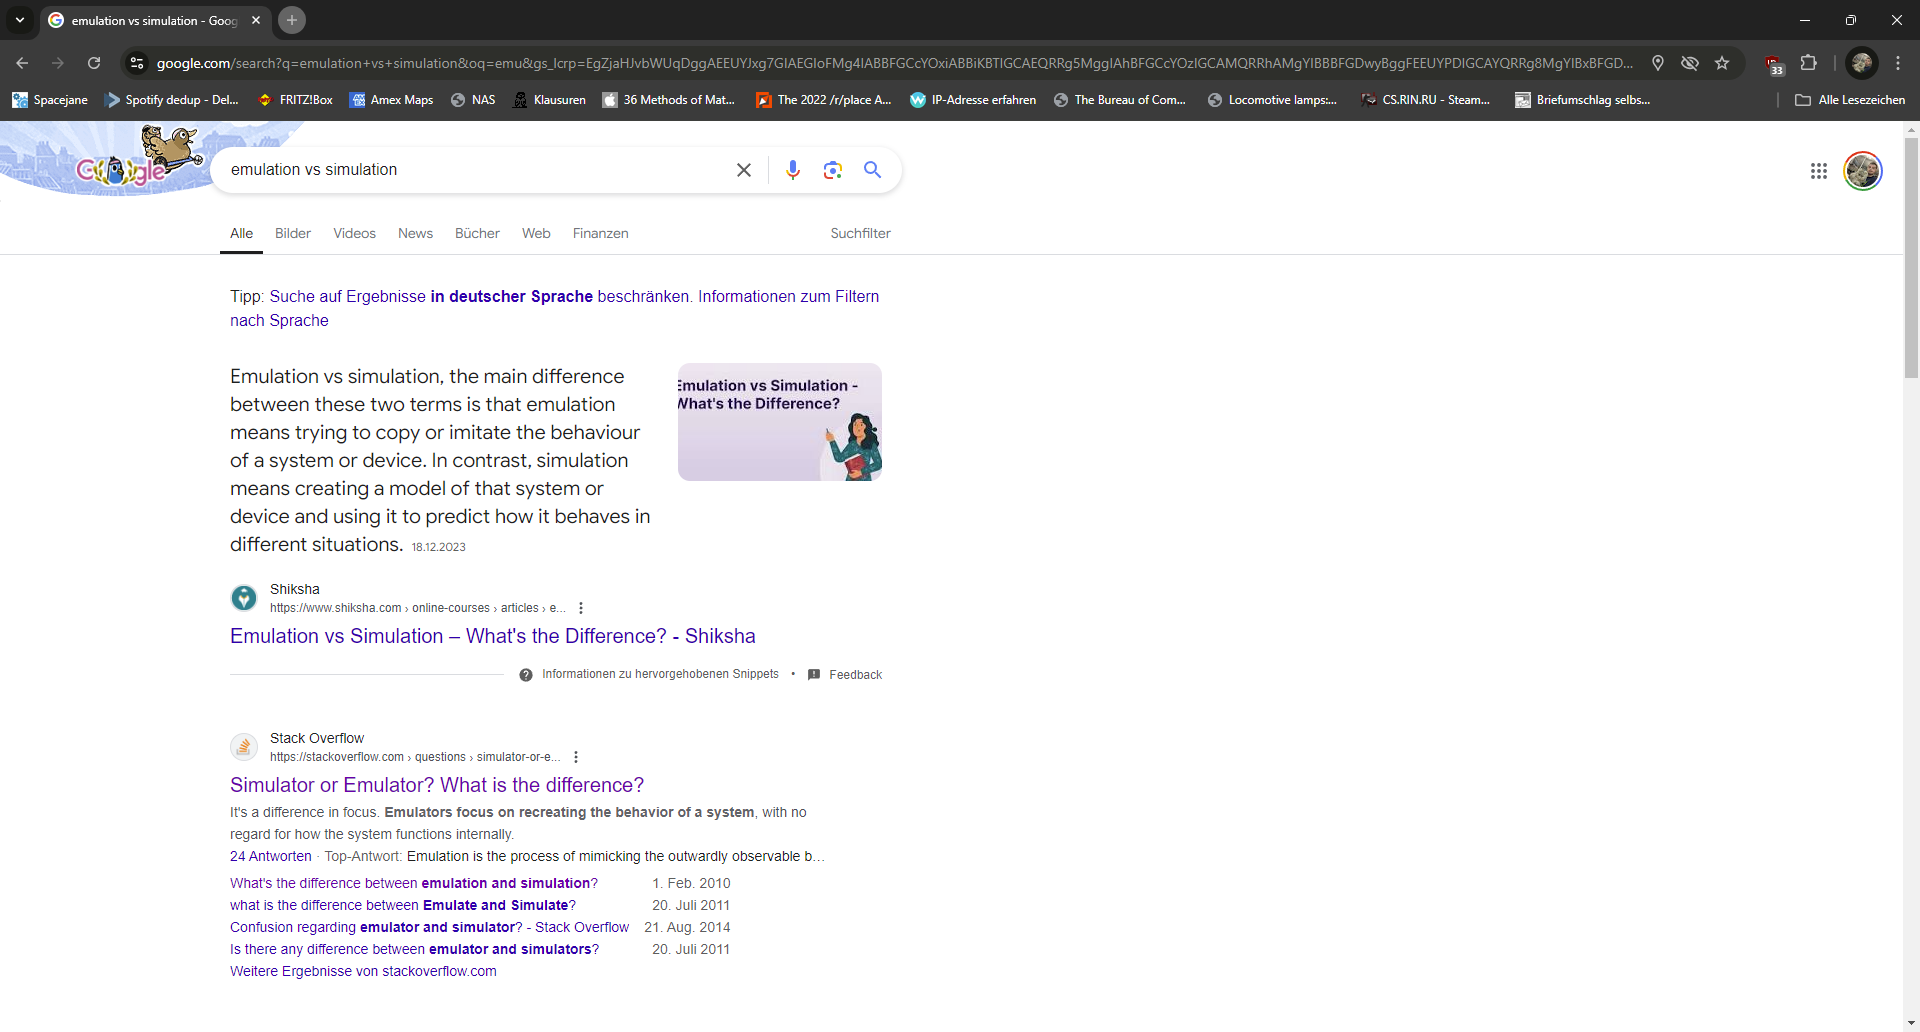
\includegraphics[width=\textwidth]{images/StackOverflow}
  \caption{The results when searching the difference between Simulation and Emulation.}
  \label{fig:Google_SO}
\end{figure}

\end{document}
